

\tikzset{every picture/.style={line width=0.75pt}} %set default line width to 0.75pt        

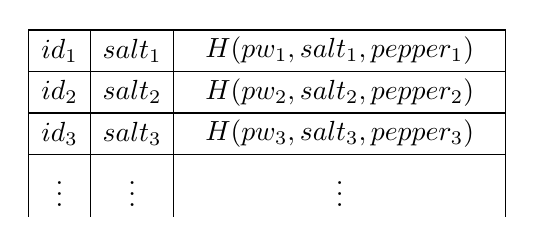
\begin{tikzpicture}[x=0.75pt,y=0.75pt,yscale=-1,xscale=1]
%uncomment if require: \path (0,94); %set diagram left start at 0, and has height of 94

%Straight Lines [id:da26114694722535137] 
\draw  [line width=0.5]  (0,0) -- (0,90) ;
%Straight Lines [id:da05297602560894288] 
\draw  [line width=0.5]  (0,0) -- (230,0) ;
%Straight Lines [id:da6769376854040197] 
\draw  [line width=0.5]  (30,0) -- (30,90) ;
%Straight Lines [id:da014741377443619808] 
\draw  [line width=0.5]  (230,0) -- (230,90) ;
%Straight Lines [id:da7062699917070598] 
\draw  [line width=0.5]  (0,20) -- (230,20) ;
%Straight Lines [id:da9213052228205383] 
\draw  [line width=0.5]  (0,40) -- (230,40) ;
%Straight Lines [id:da18806343487898314] 
\draw  [line width=0.5]  (0,60) -- (230,60) ;
%Straight Lines [id:da529477996966244] 
\draw  [line width=0.5]  (70,0) -- (70,90) ;

% Text Node
\draw (15,10) node    {$id_{1}$};
% Text Node
\draw (15,30) node    {$id_{2}$};
% Text Node
\draw (15,50) node    {$id_{3}$};
% Text Node
\draw (15,75) node    {$\vdots $};
% Text Node
\draw (150,10) node    {$H( pw_{1} ,salt_{1} ,pepper_{1})$};
% Text Node
\draw (50,75) node    {$\vdots $};
% Text Node
\draw (50,10) node    {$salt_{1}$};
% Text Node
\draw (50,30) node    {$salt_{2}$};
% Text Node
\draw (50,50) node    {$salt_{3}$};
% Text Node
\draw (150,30) node    {$H( pw_{2} ,salt_{2} ,pepper_{2})$};
% Text Node
\draw (150,50) node    {$H( pw_{3} ,salt_{3} ,pepper_{3})$};
% Text Node
\draw (150,75) node    {$\vdots $};


\end{tikzpicture}